\documentclass[10pt]{beamer}

\usetheme[progressbar=frametitle]{metropolis}
\usepackage{appendixnumberbeamer}

% ===================
% Metropolis BrownU Theme
% https://github.com/vskbellala/metropolis-brown
\usepackage{metropolisbrown}
% ===================

\usepackage{booktabs}
\usepackage[scale=2]{ccicons}

\usepackage{pgfplots}
\usepgfplotslibrary{dateplot}

\usepackage{xspace}
\newcommand{\themename}{\textbf{\textsc{metropolis}}\xspace}

\title{An Introduction to Minimum Principle}
%\subtitle{A modern beamer theme -- with a twist!}
% \date{\today}
\date{2024/07/24}
\author{Nuthasith (Nat) Gerdpratoom}
\institute{Control \& Optimization Laboratory}
\titlegraphic{\hfill\href{https://brown.edu}{
\includegraphics[height=2cm]{KU_en.png}}}

\begin{document}

\maketitle

\begin{frame}{Table of contents}
  \setbeamertemplate{section in toc}[sections numbered]
  \tableofcontents%[hideallsubsections]
\end{frame}

\section{Minimum Principle and Lagrange Multipliers}

\begin{frame}{Lagrange Multipliers in Finite Dimensions}
  Consider an optimization problem with constraint \( g(x) = \mathbf{0} \), where \(g:\mathbb{R}^{m}\rightarrow \mathbb{R}^{d}\):
  \[
    \begin{aligned}
      &\min_x V(x) \\
      &\text{s.t. } g(x) = \mathbf{0}
    \end{aligned}
  \]
  In constrained optimization in \( \mathbb{R}^m \), we use Lagrange multipliers:
  \[
  \hat{V}(x, p) = V(x) + p^T g(x)
  \]
  where \( p \) is a Lagrange multiplier. If \( x^0, p^0 \) is a stationary point, then:
  \[
  \begin{aligned}
    \nabla_x \hat{V}(x^0, p^0) &= \nabla_x V(x^0) + \nabla_x g(x^0) p^0 = \mathbf{0}\\
    \nabla_p \hat{V}(x^0, p^0) &= g(x^0) = \mathbf{0}
  \end{aligned}
  \]
  \end{frame}

\begin{frame}{Lagrange Multipliers in Finite Dimensions}
  \begin{figure}
      \centering
      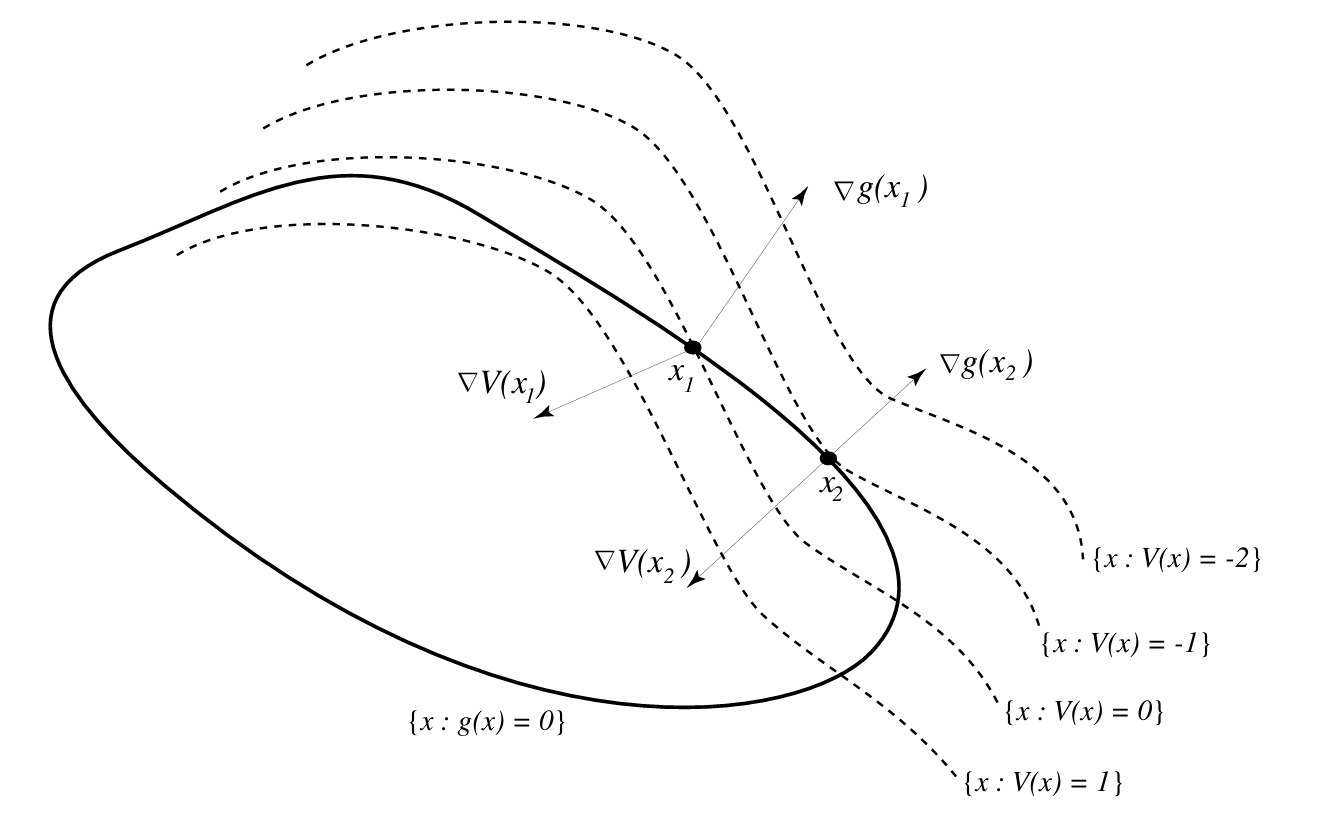
\includegraphics[width=0.8\textwidth]{photos/1.png}
      \caption{An optimization problem in \( \mathbb{R}^2 \) with a single constraint, $g(x)=0$.}
  \end{figure}
  \[
    \begin{aligned}
      \nabla_x \hat{V}(x^0, p^0) &= \nabla_x V(x^0) + \nabla_x g(x^0) p^0 = \mathbf{0}\\
      \nabla_p \hat{V}(x^0, p^0) &= g(x^0) = \mathbf{0}
    \end{aligned}
  \]
\end{frame}  

\begin{frame}{Generalizing to Infinite Dimensions}
  To generalize this to functional minimization, suppose that $F$ is a functional on $D^{r}[t_0,t_1]$, $F(z)$ is a real number, and $z \in D^{r}[t_0,t_1]$.
  We define the directional derivative:
  \[
    D_\eta F(z) = \lim_{\epsilon \to 0} \frac{F(z + \epsilon \eta) - F(z)}{\epsilon}
  \]
  A function \( z_0 \) is a stationary point of \( F \) if \( D_\eta F(z_0) = 0 \) for any \( \eta \).
  \begin{figure}
    \centering
    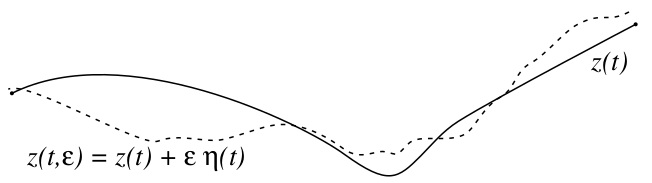
\includegraphics[width=0.7\textwidth]{photos/2.png}
    \caption{A Perturbation of function \(z\in D[t_{0},t_{1}]\)}
  \end{figure}
\end{frame}

\begin{frame}{Steps to Extend the Lagrange Multiplier Method}
  Let us consider a constrained functional optimization problem:
  \[
    \begin{aligned}
      &\min_u V(x,u)=\int \ell d \tau + m \\
      &\text{s.t. } \dot{x}-f=\mathbf{0}, \quad x\in D^{n}[t_{0},t_{1}], u \in D^{m}[t_{0},t_{1}].
    \end{aligned}
  \]
  \begin{enumerate}
      \item \textbf{Append state equations:} Define a new cost functional including the state dynamics:
      \[
      \hat{V}(x, u) = \int_{t_0}^{t_1} \ell \, dt + m(x(t_1)) + \int_{t_0}^{t_1} p^T (f - \dot{x}) \, dt
      \]
      \item \textbf{Integration by parts:} Eliminate the derivative of \( x \):
      \[
      \int_{t_0}^{t_1} p^T \dot{x} \, dt = p^T x |_{t_0}^{t_1} - \int_{t_0}^{t_1} \dot{p}^T x \, dt
      \]
  \end{enumerate}
\end{frame}

\begin{frame}{Steps to Extend the Lagrange Multiplier Method (cont.)}
  \begin{enumerate}
      \setcounter{enumi}{2}
      \item \textbf{Define the Hamiltonian:}
      \[
      H(x, p, u, t) := \ell(x, u, t) + p^T f(x, u, t)
      \]
      \[
        \begin{aligned}
          \hat{V}(x, u) = &\int_{t_0}^{t_1} H(x, p, u, t) \, dt + \int_{t_0}^{t_1}\dot{p}^{\top}xdt \\ 
          &+ p^{\top}(t_0)x(t_0) - p^{\top}(t_1)x(t_1) + m(x(t_1))
        \end{aligned}
      \]
      \item \textbf{Compute variations:} For perturbations \( x(t, \epsilon) = x^\circ(t) + \epsilon \eta(t) \) and \( u(t, \delta) = u^\circ(t) + \delta \psi(t) \), let \(\hat{V}(\epsilon)=\hat{V}(x^{\circ}+\epsilon \eta,u^{\circ}) \), and \(\hat{V}(\delta)\)=\(\hat{V}(x^{\circ},u^{\circ}+\delta \psi)\).
      \[
      \begin{aligned}
        &\frac{d}{d\epsilon} \hat{V}(\epsilon) = \int_{t_0}^{t_1} \frac{\partial}{\partial x} H(x^\circ, p, u^\circ, t) \eta(t) \, dt + \int_{t_0}^{t_1} \dot{p}^T \eta(t) \, dt \\
        &- p^T(t_1) \eta(t_1) + p^T(t_0) \eta(t_0) + \frac{\partial}{\partial x} m(x^\circ(t_1)) \eta(t_1) = 0.
      \end{aligned}
      \]
      Similarly, by considering perturbations in \( u^{\circ} \):
      \[
         \frac{d}{d\delta} \hat{V}(\delta) =\int_{t_0}^{t_1}\frac{\partial}{\partial u}H(x^{\circ},p,u^{\circ},t)\psi(t)dt=0
      \]
  \end{enumerate}
\end{frame}

\begin{frame}{Steps to Extend the Lagrange Multiplier Method (cont.)}
  \begin{enumerate}
    \setcounter{enumi}{3}
    \item \textbf{Compute variations:} Determine perturbations in \(x^{\circ}\):
    \[
    \begin{aligned}
      &\int_{t_0}^{t_1} \frac{\partial}{\partial x} H(x^\circ, p, u^\circ, t) \eta(t) \, dt + \int_{t_0}^{t_1} \dot{p}^T \eta(t) \, dt \\
      &- p^T(t_1) \eta(t_1) + p^T(t_0) \eta(t_0) + \frac{\partial}{\partial x} m(x^\circ(t_1)) \eta(t_1) = 0.
    \end{aligned}
    \]
    Similarly, by considering perturbations in \( u^{\circ} \):
    \[
       \int_{t_0}^{t_1}\frac{\partial}{\partial u}H(x^{\circ},p,u^{\circ},t)\psi(t)dt=0
    \]
    \item \textbf{Derive necessary conditions:} From the variations, derive the equations:
    \[
    \dot{p} = -\nabla_x H, \quad p(t_1) = \nabla_x m(x(t_1))
    \]
    \[
    \nabla_u H = \mathbf{0}
    \]
\end{enumerate}
\end{frame}

\begin{frame}{Deriving the Minimum Principle}
  Combine the steps to derive the Minimum Principle. If \( u^\circ \) is optimal, there exists a costate \( p(t) \) such that:
  \[
  u^\circ(t) \in \arg \min_u H(x^\circ(t), p(t), u, t)
  \]
  The state and costate satisfy:
  \[
  \dot{x}^\circ = \nabla_p H, \quad \dot{p} = -\nabla_x H
  \]
  with boundary conditions:
  \[
  x(t_0) = x_0, \quad p(t_1) = \nabla_x m(x(t_1))
  \]
\end{frame}
  
\section{The Penalty Approach}
  
\begin{frame}[fragile]{The Penalty Approach}
  Another approach to the Minimum Principle involves relaxing the hard constraint \( \dot{x} - f = 0 \), and instead imposing a large, yet "soft" constraint by  definiong the cost function:
  \[
  \hat{V}(x, u) = \int_{t_0}^{t_1} \ell(x(t), u(t), t) \, dt + \frac{k}{2} \int_{t_0}^{t_1} |\dot{x}(t) - f(x(t), u(t), t)|^2 \, dt + m(x(t_1))
  \]
  If \( (x_k, u_k) \) minimizes \( \hat{V}_k \), and letting \( (x^\circ, u^\circ) \) denote a solution to the original problem:
  \[
  \hat{V}_k(x_k, u_k) \leq \hat{V}_k(x^\circ, u^\circ) = V^\circ
  \]
  Assuming \( \ell \) and \( m \) are positive, subtracting the left side of the above inequality gives the uniform bound:
  \[
  \int_{t_0}^{t_1} |\dot{x}(t) - f(x(t), u(t), t)|^2 \, dt \leq \frac{2}{k} V^\circ
  \]
\end{frame}
  
\begin{frame}[fragile]{Implications for Large \( k \)}
  As \( k \) becomes large, the term \( \frac{k}{2} \int_{t_0}^{t_1} |\dot{x}(t) - f(x(t), u(t), t)|^2 \, dt \) ensures that \( \dot{x}(t) \approx f(x(t), u(t), t) \):
  \[
    \int_{t_0}^{t_1} |\dot{x}(t) - f(x(t), u(t), t)|^2 \, dt \rightarrow 0 \text{ as } k \rightarrow \infty
  \]
  Thus, for large \( k \), the pair \( (x_k, u_k) \) will approximately satisfy the differential equation \( \dot{x} = f \).
\end{frame}
  
\begin{frame}[fragile]{Perturbation Analysis}
  If we perturb \( x_k \) to form \( x_k + \epsilon \eta \) and define \( \hat{V}(\epsilon) = \hat{V}(x_k + \epsilon \eta, u_k) \), then we must have:
  \[
  \frac{d}{d\epsilon} \hat{V}(\epsilon) \bigg|_{\epsilon=0} = 0
  \]
  Using the definition of \( \hat{V} \), we get:
  \[
  \begin{aligned}
    \hat{V}(\epsilon) = &\int_{t_0}^{t_1} \ell(x_k(t) + \epsilon \eta(t), u_k(t), t) \, dt + m(x_k(t_1) + \epsilon \eta(t_1)) \\
    &+ \frac{k}{2} \int_{t_0}^{t_1} |\dot{x}_k(t) + \epsilon \dot{\eta}(t) - f(x_k(t) + \epsilon \eta(t), u_k(t), t)|^2 \, dt
  \end{aligned}
  \]
\end{frame}
  
\begin{frame}[fragile]{Computing the Derivative}
  The derivative of this expression with respect to \( \epsilon \) can be computed as follows:
  \[
    \begin{aligned}
      \frac{d}{d\epsilon} \hat{V}(0) &= \int_{t_0}^{t_1} \frac{\partial \ell}{\partial x} (x_k(t), u_k(t), t) \eta(t) \, dt \\
      &+ k \int_{t_0}^{t_1} (\dot{x}_k(t) - f(x_k(t), u_k(t), t))^T [\dot{\eta}(t) - \frac{\partial f}{\partial x} (x_k(t), u_k(t), t) \eta(t)] \, dt \\
      &+ \frac{\partial m}{\partial x} (x_k(t_1)) \eta(t_1) \\
      & = 0
    \end{aligned}
  \]
\end{frame}
  
\begin{frame}[fragile]{Computing the Derivative (cont.)}
  To eliminate the derivative term \( \dot{\eta} \), we integrate by parts:
  \[
  \begin{aligned}
    &\int_{t_0}^{t_1} \left\{ \frac{\partial \ell}{\partial x} (x_k(t), u_k(t), t) + p_k(t)^T \frac{\partial f}{\partial x} (x_k(t), u_k(t), t) + \frac{d}{dt} \left( p_k(t)^T \right) \right\} \eta(t) \, dt \\
    &- p_k(t_1)^T \eta(t_1) + \frac{\partial m}{\partial x} (x_k(t_1)) \eta(t_1) \\
    & = 0
  \end{aligned}
  \]
  where we have set \( p_k(t) = -k (\dot{x}_k(t) - f(x_k(t), u_k(t), t)) \).
\end{frame}

\begin{frame}[fragile]{Resulting Equations}
  Since \( \eta \) is arbitrary, we have:
  \[
    \begin{aligned}
      \mathbf{0} &= \frac{d}{dt} \left( p_k(t)^T \right) + \frac{\partial \ell}{\partial x} (x_k(t), u_k(t), t) + p_k(t)^T \frac{\partial f}{\partial x} (x_k(t), u_k(t), t) \\
      \mathbf{0} &= \frac{d}{dt} \left( p_k(t)^T \right) + \frac{\partial H}{\partial x} (x_k(t), p_k(t), u_k(t), t) \\
      \dot{p}_{k} &= -\nabla_x H
    \end{aligned}
  \]
  with the boundary condition:
  \[
    p_k(t_1) = \nabla_x m(x_k(t_1))
  \]
  Considering perturbations in \( u \) gives the equation:
  \[
    \nabla_u H (x_k(t), p_k(t), u_k(t), t) = \mathbf{0}
  \]
  This is a weak form of the Minimum Principle for the perturbed problem.
\end{frame}

\section{Application to LQR}
  
\begin{frame}[fragile]{Application to LQR}
  The LQR problem tests the Minimum Principle's utility for constructing optimal policies. Consider the general LTI model with quadratic cost:
  \[
  \dot{x} = Ax + Bu
  \]
  \[
  V = \int_{t_0}^{t_1} (x^T Q x + u^T R u) \, dt + x^T(t_1) M x(t_1)
  \]
\end{frame}

\begin{frame}[fragile]{Solving the LQR Problem}
  The Hamiltonian:
  \[
  H = x^T Q x + u^T R u + p^T (Ax + Bu)
  \]
  Control can be computed through:
  \[
  \nabla_u H = 0 \Rightarrow u = -\frac{1}{2} R^{-1} B^T p
  \]
  Resulting in:
  \[
  \dot{x} = Ax + Bu = Ax - \frac{1}{2} BR^{-1} B^T p
  \]
  Through the expression \( \nabla_x H = 2Qx + A^T p \), we find that \( \dot{p} \) is:
  \[
  \dot{p} = -\nabla_x H = -2Q x - A^T p
  \]
\end{frame}
  
\begin{frame}[fragile]{Solving the LQR Problem (cont.)}
  The equations form the coupled set of differential equations:
  \[
  \begin{pmatrix}
  \dot{x} \\
  \dot{p}
  \end{pmatrix}
  =
  \begin{pmatrix}
  A & -\frac{1}{2} BR^{-1} B^T \\
  -2Q & -A^T
  \end{pmatrix}
  \begin{pmatrix}
  x \\
  p
  \end{pmatrix}
  \]
  with boundary conditions:
  \[
  x(t_0) = x_0
  \]
  \[
  p(t_1) = \nabla_x m(x_k(t_1)) = 2Mx(t_1)
  \]
  If we scale \( p \) by defining \( \lambda = \frac{1}{2} p \), we get:
  \[
  \begin{pmatrix}
  \dot{x} \\
  \dot{\lambda}
  \end{pmatrix}
  =
  \begin{pmatrix}
  A & -BR^{-1} B^T \\
  -Q & -A^T
  \end{pmatrix}
  \begin{pmatrix}
  x \\
  \lambda
  \end{pmatrix} = \mathcal{H}   \begin{pmatrix}
    x \\
    \lambda
    \end{pmatrix}
  \]
  with the optimal control:
  \[
  u^\circ(t) = -R^{-1} B^T \lambda(t)
  \]
\end{frame}

\begin{frame}[fragile]{Solving the ODE}
  This ODE can be solved using the \textit{sweep method}. Suppose that \( \lambda(t) = P(t)x(t) \). Then:
  \[
  \dot{\lambda} = \dot{P} x + P (Ax + Bu)
  \]
  Substituting \( u^\circ = -R^{-1} B^{\top} \lambda = -R^{-1} B^{\top} P x \) gives:
  \[
  \dot{\lambda} = \dot{P} x + P (Ax - BR^{-1} B^{\top} P x)
  \]
  From the coupled ODE with \(\mathcal{H}\) above, we also have:
  \[
  \dot{\lambda} = -Qx - A^{\top} \lambda = -Qx - A^{\top} P x
  \]
  Equating the two expressions for \( \dot{\lambda} \) gives the Riccati Differential Equation:
  \[
  \dot{P} x + P (Ax - BR^{-1} B^{\top} P x) = -Qx - A^{\top} P x
  \]
\end{frame}

\begin{frame}[fragile]{Boundary Condition}
  The boundary condition for \( \lambda \) is:
  \[
  \lambda = \frac{1}{2} p = \frac{1}{2} \nabla_x m(x(t_1)) \implies P(t_1) = M
  \]
  Solving for \( P(t) \) gives \( \lambda(t) \), which in turn gives \( p(t) \).
\end{frame}

\section{Nonlinear Examples}

\begin{frame}[fragile]{Minimum Principle with Constraints}
  \textbf{Theorem 11.2 (Minimum Principle with constraints)}. Suppose that \( x(t_1) \) is free, \( t_1 \) is fixed, and suppose that \( u^\circ \) is a solution to the optimal control problem: 
  \[
    V^\circ = \min_{u \in \mathcal{U}} V(u)
  \]
  We then have
  \begin{itemize}
      \item[(a)] There exists a costate vector \( p(t) \) such that
      \[
        u^\circ (t) = \arg \min_{u \in \mathcal{U}} H(x^\circ (t), p(t), u, t).
      \]
  
      \item[(b)] The pair \( (p, x^\circ) \) satisfy the 2-point boundary value problem:
      \begin{align*}
        \dot{x}^\circ(t) &= \nabla_p H(x^\circ(t), p(t), u^\circ(t), t) \quad \left( = f(x^\circ(t), u^\circ(t), t) \right) \\
        \dot{p}(t) &= -\nabla_x H(x^\circ(t), p(t), u^\circ(t), t),
      \end{align*}
      with the two boundary conditions
      \[
        x(t_0) = x_0; \quad p(t_1) = \frac{\partial}{\partial x} m(x(t_1), t).
      \]
  \end{itemize}
\end{frame}
  
\begin{frame}[fragile]{Example 11.5.1: Bilinear System}
  Consider the control of a bilinear system, defined by the differential equation:
  \[
  \dot{x} = ux, \quad x(0) = x_0 > 0, \quad 0 \le u(t) \le 1
  \]
  Suppose the goal is to make \( x \) large while keeping the derivative of \( x \) small on average. The cost criterion is:
  \[
    V(u) = \int_0^{t_1}\dot{x}(\tau)-x(\tau)d\tau = \int_0^{t_1} [u(\tau) - 1]x(\tau) \, d\tau
  \]
  The Hamiltonian becomes:
  \[
    H(x, p, u, t) = pf+\ell = x \{ u(p + 1) - 1 \}
  \]
\end{frame}
  
\begin{frame}[fragile]{Optimal Control of Bilinear System}
  By the Minimum Principle:
  \[
    \begin{aligned}
      H(x, p, u, t) &= x \{ u(p + 1) - 1 \} \\
      \nabla_u H &= x(p + 1)
    \end{aligned}
  \]
  Since \( x^{\circ}(t) > 0 \) for all $t$, the minimization leads to:
  \[
  u^\circ(t) = \begin{cases}
  1 & \text{if } p(t) + 1 < 0 \\
  0 & \text{if } p(t) + 1 > 0 \\
  \text{unknown} & \text{if } p(t)+1 = 0
  \end{cases}
  \]
\end{frame}
  
\begin{frame}[fragile]{Costate and State Equations}
  The costate and state variables satisfy:
  \[
  \dot{p} = -(p + 1)u^\circ + 1
  \]
  \[
  \dot{x}^\circ = u^\circ x^\circ
  \]
  with the boundary conditions:
  \[
  x^\circ(0) = x_0, \quad p(t_1) = 0
  \]
\end{frame}
  
\begin{frame}[fragile]{Solving the Differential Equations}
  If \( t = t_1 \), then \( p(t) + 1 = 1 > 0 \) so \( u^\circ(t) = 0 \). By continuity, if \( t \approx t_1 \), then \( p(t) > 0 \), so \( u^\circ(t) = 0 \) and:
  \[
  \dot{p}(t) = 1 \quad \text{for } t \approx t_1 \implies p(t) = t - t_1
  \]
  For \( t < t_1 - 1 \), we have \( p(t) + 1 < 0 \) so \( u^\circ(t) = 1 \) and:
  \[
  \dot{p} = -p \quad \text{for } t < t_1 - 1 \implies p(t) = -e^{-t + t_1 - 1}
  \]
\end{frame}
  
\begin{frame}[fragile]{Bang-Bang Control}
  The optimal control is bang-bang:
  \[
  u(t) = \begin{cases}
  1 & \text{if } t < t_1 - 1 \\
  0 & \text{if } t > t_1 - 1
  \end{cases}
  \]
  The optimal state trajectory is:
  \[
  \dot{x}^\circ(t) = \begin{cases}
  x^\circ(t) & \text{if } t < t_1 - 1 \\
  0 & \text{if } t > t_1 - 1
  \end{cases}
  \]
  \[
  x^\circ(t) = \begin{cases}
  x_0 e^t & \text{if } t < t_1 - 1 \\
  x_0 e^{t_1 - 1} & \text{if } t > t_1 - 1
  \end{cases}
  \]
\end{frame}
  
\begin{frame}[fragile]{Minimum Principle with Constraints}
  Suppose \( x(t_1) \) is free, \( t_1 \) is fixed, and \( u^\circ \) is a solution to the optimal control problem (11.1) under the constraint \( u \in U \). The Minimum Principle with constraints states:
  \begin{enumerate}
      \item There exists a costate vector \( p(t) \) such that \( u^\circ(t) = \arg \min_{u \in U} H(x^\circ(t), p(t), u, t) \).
      \item The pair \( (p, x^\circ) \) satisfy the 2-point boundary value problem.
  \end{enumerate}
\end{frame}
  
\begin{frame}[fragile]{Example 11.5.1 with Constraints}
  Consider the bilinear system:
  \[
  \dot{x} = ux, \quad x(0) = x_0 > 0, \quad 0 \le u(t) \le 1
  \]
  with the cost criterion:
  \[
  V(u) = \int_0^{t_1} [u(\tau) - 1] x(\tau) \, d\tau
  \]
  The Hamiltonian:
  \[
  H(x, p, u, t) = x \{ u(p + 1) - 1 \}
  \]
  Optimal control:
  \[
  u^\circ(t) = \begin{cases}
  1 & \text{if } p(t) + 1 < 0 \\
  0 & \text{if } p(t) + 1 > 0
  \end{cases}
  \]
\end{frame}
  
\begin{frame}[fragile]{Costate and State Variables for Constrained Problem}
  The costate and state variables satisfy:
  \[
  \dot{p} = -(p + 1) u^\circ + 1
  \]
  \[
  \dot{x} = u^\circ x
  \]
  with boundary conditions \( x^\circ(0) = x_0 \), \( p(t_1) = 0 \).
\end{frame}
  
\begin{frame}[fragile]{Solving the Constrained Problem}
  If \( t \approx t_1 \):
  \[
  p(t) = t - t_1
  \]
  For \( t < t_1 - 1 \):
  \[
  p(t) = -e^{-t + t_1 - 1}
  \]
  The optimal control is bang-bang:
  \[
  u(t) = \begin{cases}
  1 & t < t_1 - 1 \\
  0 & t > t_1 - 1
  \end{cases}
  \]
\end{frame}
  
\begin{frame}[fragile]{Optimal State Trajectory for Constrained Problem}
  The optimal state trajectory:
  \[
  \dot{x}^\circ(t) = \begin{cases}
  x^\circ(t) & t < t_1 - 1 \\
  0 & t > t_1 - 1
  \end{cases}
  \]
  \[
  x^\circ(t) = \begin{cases}
  x_0 e^t & t < t_1 - 1 \\
  x_0 e^{t_1 - 1} & t > t_1 - 1
  \end{cases}
  \]
\end{frame}
  
\begin{frame}[fragile]{Minimum Principle with Final Value Constraints}
  Suppose \( t_0, t_1, x(t_0) = x_0 \), and \( x(t_1) = x_1 \) are prespecified. The Minimum Principle with final value constraints states:
  \begin{enumerate}
      \item There exists a costate vector \( p(t) \) such that \( u^\circ(t) = \arg \min_u H(x^\circ(t), p(t), u, t) \).
      \item The pair \( (p, x^\circ) \) satisfy the 2-point boundary value problem.
  \end{enumerate}
\end{frame}
  
\begin{frame}[fragile]{Example 11.5.2: LQR Problem with Terminal State}
  Consider the LQR problem with the terminal state specified. The cost criterion is:
  \[
  V = \frac{1}{2} \int_0^{t_1} (x^T Q x + u^T R u) \, dt, \quad R > 0, Q \ge 0
  \]
  The Hamiltonian:
  \[
  H = p (A x + B u) + \frac{1}{2} (x^T Q x + u^T R u)
  \]
  The optimal control:
  \[
  u^\circ(t) = -R^{-1} B^T p(t)
  \]
\end{frame}
  
\begin{frame}[fragile]{Costate Equation for LQR Problem}
  The costate vector satisfies the differential equation:
  \[
  \dot{p}(t) = -\frac{\partial H}{\partial x} = -p^T A - x^T Q
  \]
  \[
  (x, p) = \begin{pmatrix}
  A & -BR^{-1}B^T \\
  -Q & -A^T
  \end{pmatrix} \begin{pmatrix}
  x \\
  p
  \end{pmatrix}
  \]
  with boundary conditions:
  \[
  x(t_0) = x_0, \quad x(t_1) = x_1
  \]
\end{frame}
  
\begin{frame}[fragile]{State Transition Matrix}
  Let \( \psi(t, \tau) \) denote the state transition matrix:
  \[
  \frac{d}{dt} \psi(t, \tau) = H(t) \psi(t, \tau), \quad \psi(t, t) = I
  \]
  Decompose \( \psi(t, \tau) \) as:
  \[
  \psi(t, \tau) = \begin{pmatrix}
  \psi_{11}(t, \tau) & \psi_{12}(t, \tau) \\
  \psi_{21}(t, \tau) & \psi_{22}(t, \tau)
  \end{pmatrix}
  \]
\end{frame}
  
\begin{frame}[fragile]{Solving for Optimal Control}
  Compute the initial condition \( p(t_0) = p_0 \) to find \( p(t) \) for all \( t \):
  \[
  x_1 = x(t_1) = \psi_{11}(t_1, t_0) x_0 + \psi_{12}(t_1, t_0) p_0
  \]
  Assuming \( \psi_{12}(t_1, t_0) \) is invertible, we have:
  \[
  p_0 = \psi_{12}(t_1, t_0)^{-1} (x_1 - \psi_{11}(t_1, t_0) x_0)
  \]
\end{frame}
  
\begin{frame}[fragile]{Optimal Control and State Trajectory}
  For all \( t \):
  \[
  p(t) = \psi_{21}(t, t_0) x_0 + \psi_{22}(t, t_0) p_0
  \]
  The optimal control is:
  \[
  u^\circ(t) = -R^{-1} B^T p(t)
  \]
  The optimal state trajectory is:
  \[
  x^\circ(t) = \psi_{11}(t, t_0) x_0 + \psi_{12}(t, t_0) p_0, \quad t \ge t_0
  \]
\end{frame}
  
\begin{frame}[fragile]{Minimum Principle with Free Terminal Time}
  Suppose \( t_0, x(t_0) = x_0 \) are fixed, and some components of \( x(t_1) \) are specified. The Minimum Principle with free terminal time states:
  \begin{enumerate}
      \item There exists a costate vector \( p(t) \) such that \( u^\circ(t) = \arg \min_u H(x^\circ(t), p(t), u, t) \).
      \item The pair \( (p, x^\circ) \) satisfy the 2-point boundary value problem with modified boundary conditions.
      \item The unspecified terminal time \( t_1 \) satisfies:
      \[
      \frac{\partial m}{\partial t}(x^\circ(t_1), t) + H(x^\circ(t_1), p(t_1), u^\circ(t_1), t_1) = 0
      \]
  \end{enumerate}
\end{frame}
  
\begin{frame}[fragile]{Example 11.5.3: Minimum Time Problem}
  Consider a single input linear state space model:
  \[
  \dot{x} = Ax + bu
  \]
  We wish to find \( u^\circ \) which drives \( x \) from \( x(0) = x_0 \) to \( x(t_1) = x_1 \) in minimum time, under the constraint \( |u(t)| \le 1 \). The cost criterion is:
  \[
  V(u) = t_1 = \int_0^{t_1} 1 \, dt
  \]
  The Hamiltonian is:
  \[
  H = 1 + p^T(Ax + bu)
  \]
\end{frame}
  
\begin{frame}[fragile]{Bang-Bang Control Law}
  Minimizing \( H \) gives a bang-bang control law:
  \[
  u^\circ(t) = \begin{cases}
  1 & \text{if } p(t)^T b < 0 \\
  -1 & \text{if } p(t)^T b > 0
  \end{cases}
  \]
  If \( A, b \) are time-invariant and the eigenvalues of \( A \) are real, distinct, and negative, then \( p(t)^T b \) changes sign at most \( n - 1 \) times, bounding the number of switching times for the optimal control.
\end{frame}
  
\begin{frame}[fragile]{Costate Equation for Minimum Time Problem}
  The costate equation is:
  \[
  \dot{p} = -\nabla_x H = -A^T p
  \]
  Using the final time boundary condition \( H|_{t=t_1} = 0 \):
  \[
  1 + p(t_1)^T A x^\circ(t_1) + p(t_1)^T b u^\circ(t_1) = 1 + p(t_1)^T A x^\circ(t_1) - |p(t_1)^T b| = 0
  \]
\end{frame}
  
\begin{frame}[fragile]{Example: Double Integrator}
  Consider the double integrator \( \ddot{y} = u \):
  \[
  A = \begin{pmatrix} 0 & 1 \\ 0 & 0 \end{pmatrix}, \quad b = \begin{pmatrix} 0 \\ 1 \end{pmatrix}
  \]
  The optimal control is:
  \[
  u^\circ(t) = -\text{sgn}(p(t)^T b) = -\text{sgn}(p_2(t))
  \]
\end{frame}
  
\begin{frame}[fragile]{Solving Costate Equations}
  From the costate equations, for constants \( c_1, c_2 \):
  \[
  p_1(t) = c_1, \quad p_2(t) = -c_1 t + c_2
  \]
  The optimal control is bang-bang:
  \[
  u^\circ(t) = \begin{cases}
  1 & \text{if } t < t_1 - 1 \\
  0 & \text{if } t > t_1 - 1
  \end{cases}
  \]
\end{frame}
  
\begin{frame}[fragile]{Optimal Trajectories}
  The optimal state trajectories follow quadratic paths:
  \[
  x_1(t) = \begin{cases}
  \frac{1}{2} (x_2(t))^2 + K_1 & \text{if } u^\circ(t) = 1 \\
  -\frac{1}{2} (x_2(t))^2 + K_2 & \text{if } u^\circ(t) = -1
  \end{cases}
  \]
\end{frame}
\end{document}
